\documentclass[12pt]{article}

\usepackage[bottom = 15mm]{geometry}
\usepackage[utf8]{inputenc}
\usepackage[T2A]{fontenc}
\usepackage[russian]{babel}
\usepackage{graphicx}
\usepackage{caption}
\usepackage{amssymb, gensymb, amsmath}
\usepackage{mathrsfs}
\usepackage{array, colortbl}
\usepackage{multicol}

\newcommand{\RF}{${\bf r_1}$ }
\newcommand{\RS}{${\bf r_2}$ }

\textwidth = 16 cm
\textheight = 23  cm
\oddsidemargin = 0 pt
\topmargin = -1.5 cm
\parindent = 20 pt
\parskip = 0 pt
\flushbottom


\title{{\bf Задача 4.\,2.\,5 \\ Когерентность света}}
\author{Лось Денис (группа 611)}
\date{21 февраля 2018}

\begin{document}

\maketitle

\paragraph{Основные цели работы: } настройка интерферометра, определение радиусов, длины, времени когерентности; средней длины волны и ширины спектра источника света.

\paragraph{В  работе используются: } лазер, галогенная лампа с блоком питания, объектив, оптические щели, микроскоп.

\section*{Теоритическая часть}
\par
	Рассмотрим проблему согласованности световых колебаний от источника в двух точках с координатами ${\bf r_1}$ и ${\bf r_2}$ в моменты времени $t_1$ и $t_2$. При этом световые колебания будем считать квазимонохроматическими с центральной частотой $\omega_0$, а поле будем считать скалярным, т.е. не будем учитывать эффекты, связанные с поляризацией излучения. Если поле световой волны в точке ${\bf r}$ в момент времени $t$ записать как $A({\bf r}, t) e^{iw_0t}$, то за меру когерентности световых колебаний \RF и \RSв моменты времени $t_1$ и $t_2$ выбирают нормированное среднее произведение амплитуд полей
\begin{equation}
	\gamma = \frac{\overline{A({\bf r_1}, t_1) e^{iw_0t_1} \cdot A^{*}({\bf r_2}, t_2) e^{-iw_0t_2}}}{\sqrt{\overline{|A({\bf r_1}, t_1)|^2} \cdot {\overline{|A({\bf r_2}, t_2)|^2}}}}
\end{equation}
\par
	Исследуя согласованность колебаний точек, лежащих в одной плоскости, и считатя, что случайное световое поле является однородным в пространстве и его статические характеристики не зависят от времени, придём к выводу, что функция когерентности $\gamma$ не зависит от координат \RF, \RS и моментов времени $t_1$ $t_2$, а зависит только от их разности $\rho = |{\bf \rho}| = |{\bf r_2 - r_1}|$ и $\tau = t_2 - t_1$.
\par
	Считая для выбранной пары точек интенсивность постоянной ($\overline{|A|^2}$), приведём $\gamma$ к виду
\begin{equation}
	\gamma = e^{-i w_0 \tau} \frac{\overline{A({\bf r}, t) \cdot A^{*}({\bf r + \rho}, t + \tau)}}{\overline{|A|^2}}
\end{equation}
\par
	Укажем связь между функцией когерентности $\gamma$ и видностью, при условии, что оптическая система позволяет наложить друг на друга световые поля $A({\bf r}, t) e^{iw_0t}$ и $A({\bf r + \rho}, t + \tau) e^{iw_0(t + \tau)}$ и измерить интенсивность суммарного поля
\[
	I \approx 2 |A|^2 \left[1 + |\gamma(\rho, \tau)| \cos\left(w_o \tau - \delta(\rho, \tau) \right) \right],
\]
где $\delta(\rho, \tau)$ --- фаза комплексной амплитуды функции когерентности, которая, если фиксировать расстояние между точками, при малых изменениях времени зарежки $\tau$ меняется пренебрежительно мало по сравнению с $w_0 \tau$. А следовательно, 
\begin{equation}
	V(\rho, \tau) = \frac{I_\text{max} - I_\text{min}}{I_\text{max} + I_\text{min}} = |\gamma(\rho, \tau)|
\end{equation}
\par
	Вспомним о том, что глаз может различить интерференционную картину при $V > 0.1$.
\par
	Рассмотрим некоторые частные постановки задач по определению модуля функции когерентности или видности интерференционной картины.
\begin{enumerate}
	\item
		\par
			Нас интересует когерентность в точках $A$ и $B$, причём расстояние между ними фиксировано $AB = \rho$, а поле распространяется в положительном направлении оси $z$. Смотреть рисунок 1 приложения к работе.
		\par
			Если в плоскость, в которой лежат эти точки поместить очень тонкий непрозрачный экран с отверстиями около этих точек, то падающая на экран световая волна будет испытывать дифракцию на границах отверстий, а значит, поместив на достаточно большом от этого экрана с отверстиями и параллельно ему плоскость наблюдение, мы сможем определить интенсивность интерференцинной картины, а следовательно, и её видность.
		\par
			Рассматривая источник пренебрежимо малого углового размера, помещённый в точку С,  запишем выражение для интенсивности в точке $P$, региструемой инерционным прибором (в данном случае глазом), опуская подробный его вывод
\begin{equation}
	I_P = I_0 \left[1 + \cos\left(\frac{\rho w_0}{c} \left(\varphi - \theta\right) \right) \, e^{-\left[\frac{\rho \Omega}{2 c} \left(\varphi - \theta\right) \right]^2} \right]
\end{equation}
		Здесь $\Omega$ --- ширина спектра излучения источника, $\theta$ --- угол, под которым исчточник виден из центра экрана, и $\varphi$ --- угол дифракции (показаны на рисунке 1 в приложении к работе), а $I_0 = $ const.
		\par
			На экране это выглядит как интерференционные полосы с меняющейся контрастностью $e^{-\left[\frac{\rho \Omega}{2 c} \left(\varphi - \theta\right) \right]^2}$ картины. Угловые координаты максимумов полос
\begin{equation}
	\varphi_m = \theta + \frac{\lambda_0}{\rho}m,
\end{equation}
	где $m = 0, \pm 1, \pm 2, \dots$ --- порядок интерференции.
		\par
			Максимальный порядок наблюдаемой картины интерференции $m_\text{ког}$
\begin{equation}
	m_\text{ког} \approx \frac{\lambda_0}{\Delta \lambda}
\end{equation}		
		\par
			{\bf Длина когерентности} --- максимальная разность хода, при которой наблюдается интерференция
\begin{equation}
	\Delta_\text{ког} = m_\text{ког} \lambda_0 = \frac{\lambda_0^2}{\Delta \lambda}
\end{equation}
		\par
			{\bf Время когерентности} --- максимальное время задержки $\tau$
\begin{equation}
	\tau_\text{ког} = \frac{\Delta_\text{ког}}{c}
\end{equation}
	\item
		\par
			Если теперь вместо точечного источника возьмём тонкую нить, лежащую вдоль оси x, такую, что её угловой размер $\theta_0$ мал (так как контрастность изображения в плоскости наблюдения не должна сильно уменьшиться), а  сама она равномерно светится по длине и является абсолютно некогерентным источников света, то для интенсивности света в точке $P$ плоскости наблюдения
\begin{equation}
	I_P = I_0 \left\lbrace 1 + e^{-\left(\frac{\rho \Omega}{2 c} \varphi\right)^2} \frac{\sin \left(\frac{\rho \omega_0 \theta_0}{2 c} \right)}{\frac{\rho \omega_0 \theta_0}{2 c}} \cdot \cos \left(\frac{\rho \omega_0}{c} \varphi \right) \right\rbrace \label{f1}
\end{equation}
	\item
		\par
		Если вместо одного экрана возьмём набор экранов с разными расстояними между отверстиями, то интенсивность света в точке наблюдения будет являться функцией двух переменных расстояния между точками $\rho$ и угла дифракции $\varphi$. В этих переменных интерференционный максимум порядка $m$ будет описываться уравнением $\rho \varphi = m \lambda_0$, т.е. будет являться гиперболой.
		\par
			Контрастность интерференционной картины будет уменьшаться не только с увеличением времени задержки $\tau = \frac{\rho \varphi}{c}$, что связано с шириной спектра источника $\Omega$, но и с увеличением расстояния между точками $\rho$, что определяется конечным угловым размером нити $\theta_0$. Контрастность будет обращаться в ноль, если расстояние между отверстиями будет равно радиусу поперечной когерентности
\begin{equation}
	\rho_\text{ког} = \frac{\lambda_0}{\theta_0}
\end{equation}
	\par
		Модуль функции когерентности в переменных $\rho$ и $\tau$
\begin{equation}
	|\gamma(\rho, \tau)| = V(\rho, \tau) = e^{-\left(\frac{\Omega \tau}{2} \right)^2} \left|\frac{\sin\left(\frac{\pi \theta_0}{\lambda_0} \rho \right)}{\frac{\pi \theta_0}{\lambda_0} \rho} \right|
\end{equation}
\end{enumerate}		
\newpage
\section*{Экспериментальная установка. Описание интерферометра.}
\par
	Принципиальная схема интерферометра на рис.1. Стоит обратить внимание, что в работе вместо цилиндрической линзы Л2 используется {\bfсферическая} линза.
\begin{figure}[h!]
	\centering
	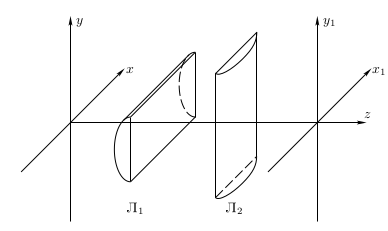
\includegraphics[width = 12cm, height = 5cm]{image1.png}
	\caption{Принципиальная схема интерферометра}	
\end{figure}	
\par
	Здесь в плоскость $(x,y)$ помещается экран, изготовленный в виде двух взаимно перпендикулярных узких щелей, плоскость $(x_1, y_1)$ является плоскостью наблюдения, а $z$ --- оптическая ось системы. На участках щелей экрана, помещённого в $(x,y)$ происходит дифракция. Для того чтобы пространственно разделить дифракционные картины от различных симметричных относительно вертикальной оси пары участков мы используем {\bf цилиндрическую линзу Л1}, ось цилиндра которого горизонтальна, а фокусное расстояние линзы $f_1$ удовлетворяет условию $\frac{1}{f_1} = \frac{1}{a} + \frac{1}{b}$, где $a + b$ --- расстояние между двумя вышеупомянутыми плоскостями. Для того чтобы совместить главные дифракционные максимумым для каждой симметричной относительно вертикальной оси пар участков мы будем использовать {\bf сферическую линзу} (мы также можем использовать цилиндрическую линзу Л2) с фокусным расстоянием $f_2 = b$. Подобная конфигурация позволяет нам получить соответствие интенсивности, получаемой с помощью интерферометра, с интенсивностью из формулы (\ref{f1}). Однако в плоскости наблюдения интерферометра изображение получается в координатах $x_1$ и $y_1$, но мы сможем перевести их в переменные $\rho$ и $\varphi$ как
\begin{equation}
	\varphi = \frac{x_1}{b} \qquad \rho = 2 \frac{a}{b}|y_1| = 2 \frac{|y_1|}{G},
\end{equation}
где $G$ --- это увеличение объектива, образованного двумя описанными выше линзами.
\noindent\rule{\textwidth}{1pt}
\par
	Так как процесс непосредственной сборки экспериментальной установки в данной работе является одним их ключевых пунктов в её выполнении , то методику измерений, а также получаемые результаты мы будем приводить по ходу её выполнения.
\noindent\rule{\textwidth}{1pt}
\section*{Ход работы. Сборка экспериментальной установки. Результаты измерений.}
\paragraph{Первоначальная сборка установки. Оценка длины волны излучения лазера.}
\par
	Соберём экспериментальную установку, показанную на рис.2. (принципиальный ход лучей лазера показан только до поляроида).
\begin{figure}[h!]
	\centering
	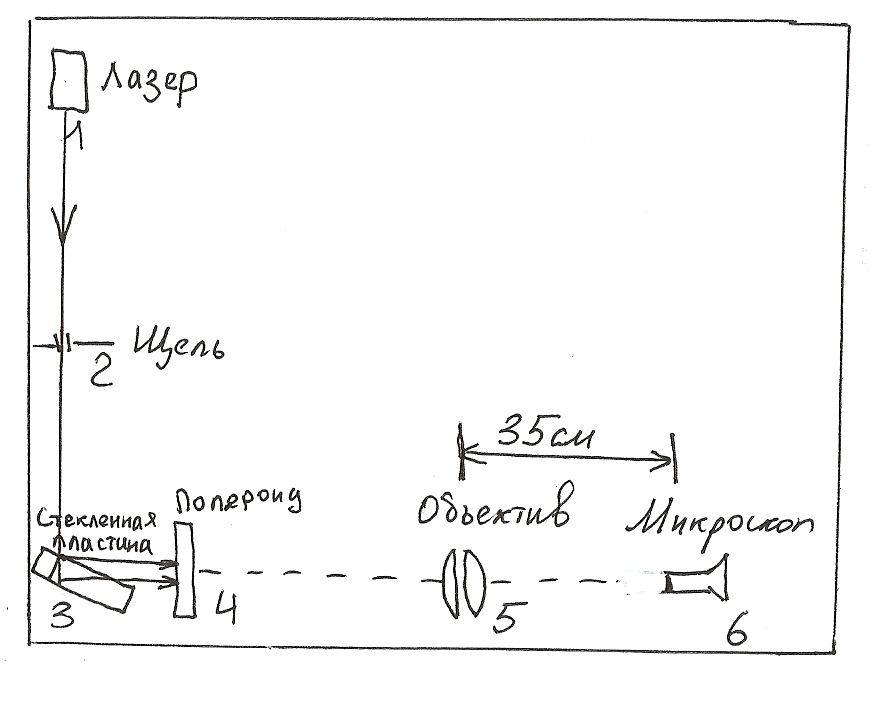
\includegraphics[width = 10cm, height = 6cm]{image3.png}
	\caption{Схема установки для оценки длины волны лазера}
\end{figure}
\par
	Ширина щели 2, установленной между стеклянной пластиной 3 и лазером 1, выбирается максимальной так, чтобы щель пропускала центральную область лазерного пятна. Объектив 4 установлен на расстоянии $b = \left(35.0 \pm 0.5\right)$ см от объектива микроскопа, что было измерено с помощью сантиметровой линейки. Стеклянная пластинка здесь используется по причине того, что получить в микроскопе картину стандартной дифракции Фраунгофера на щели без неё практически невозможно в силу малости углов схождения лучей в фокальной плоскости объектива. Благодаря отражению от плоскостей пластинки создаются два изображения оптической щели, параллельные друг другу.
\par
	В микроскоп мы будем наблюдать интерференционную картину, расстояние между полосами которой $\Delta$ мы измерим с помощью окулярной шкалы микроскопа с ценой деления $0.02$ мм. В результате получим, что $\Delta = 0.02$ мм. Расстояние между пучками $u = (9 \pm 1)$ мм, которое мы измерили с помощью миллиметровой линейки.
\par
	Длину волны лазера мы можем оценить как
\[
	\lambda _\text{лаз} \approx \frac{\Delta}{b} u = 514 \, \text{нм} 
\]
\noindent\rule{\textwidth}{1pt}
\par
	Погрешность для $\lambda_\text{лаз}$ не приводится, так как здесь нашей целью является лишь оценить, чему длина волны равна для используемого зелёного лазера. Более подробная информация приведена в выводах к работе.

\noindent\rule{\textwidth}{1pt}

\newpage
\paragraph{Определение предметной плоскости интерферометра}
\par
	Идея состоит в том, чтобы с помощью дополнительного транспаранта (стальной нити диаметром 1 мм) определить положение плоскости, куда затем будут установлены щели в виде креста. Принципиальная схема установки приведена на рис.3.
\begin{figure}[h!]
	\centering
	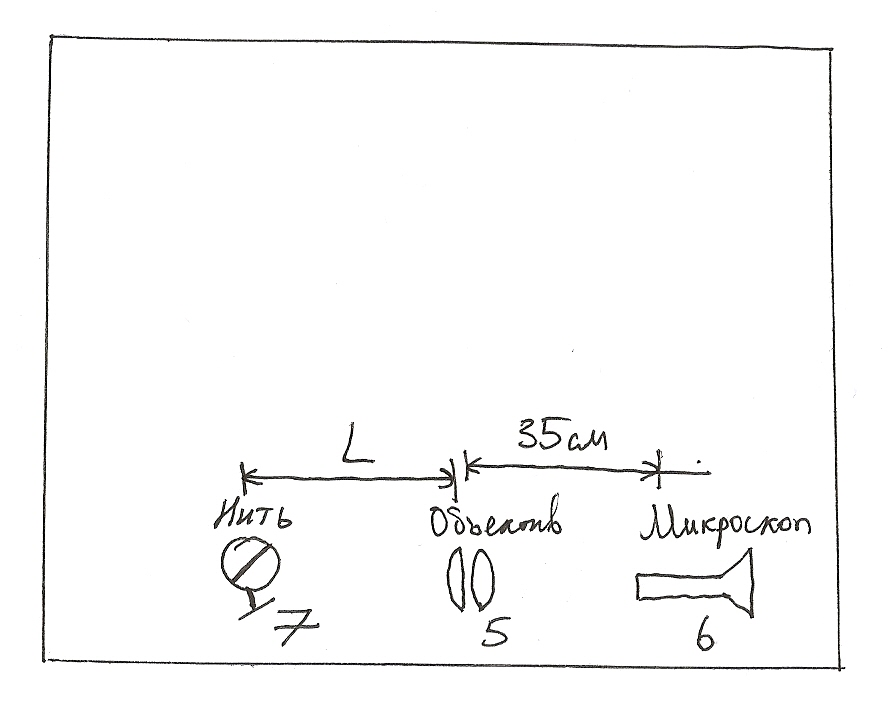
\includegraphics[width = 10cm, height = 6cm]{image2.png}
	\caption{Схема установки для определения предметной плоскости интерферометра}
\end{figure}
\par
	Перемещая транспарант вдоль оси системы, добъёмся резкого изображения нити, при этом зафиксировав расстояние $L$ между держателем нити и объективом 5. Заметим, что лишь при перемещении держателя на расстояния свыше $0.5$ см вдоль оси системы резкость изображения нити значительно ухудшается. Под значительностью ухудшения резкости здесь понимается возможность визуально разделить два положения держателя на более резкое и менее резкое изображения. В результате
\[
	L = \left(44.5 \pm 0.5 \right) \, \text{см}
\]
\par
	Измерим по окулярной шкале микроскопа видимый размер нити по вертикали
\[
	d = \left(0.66 \pm 0.01\right) \, \text{мм}
\]
\par
	Следовательно, увеличение объектива
\[
	G = \left(0.66 \pm 0.01 \right)
\]
\newpage
\paragraph{Опыты с лампой}
\par
	Соберём схему согласно рис.4.
\begin{figure}[h!]
	\centering
	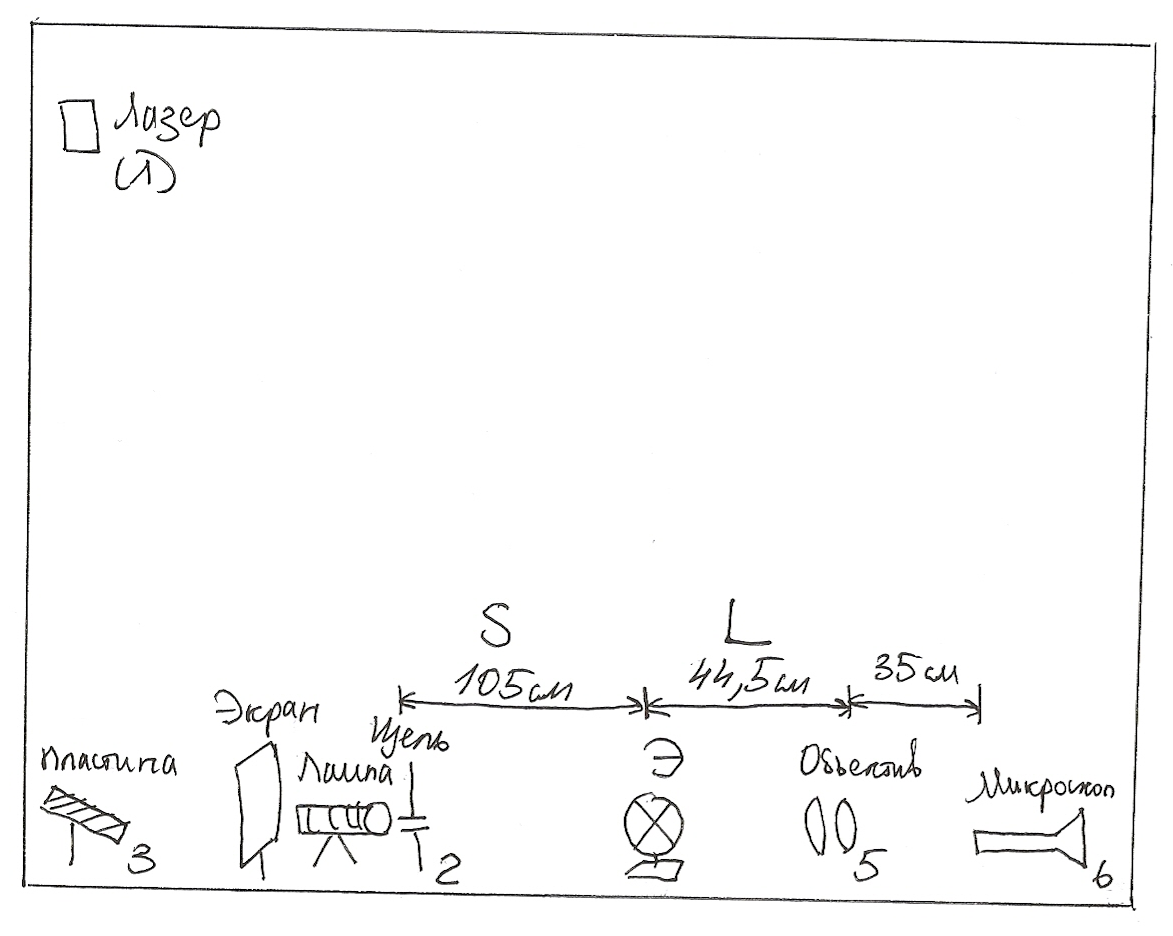
\includegraphics[width = 10cm, height = 6cm]{image4.png}
	\caption{Схема установки для проведения опытов с лампой}
\end{figure}
\par
	Здесь луч лазера используется для контроля центральности системы. После совмещения центра щелей Э, центра нити лампы и луча лазера, ставится экран и проводятся опыты с лампой.
\par
	Для нескольких значений ширины щели $d$, которая измеряется с помощью микрометрического винта, измерим радиус поперечной когерентности. Для этого будем искать положения по вертикальной оси (окулярная шкала микроскопа расположена вертикально), в которых интерференционные полосы пропадают, а потом снова возникают с увеличением их вертикальной координаты. Обозначим это вертикальное положение как $y$.
\par
	Погрешность радиуса когеренции может быть определена согласно (12) как
\[
	\Delta_\text{$\rho_\text{ког}$} = \rho_\text{ког} \cdot \sqrt{\sigma_y^2 + \sigma_G^2}
\]
\begin{table}[h!]
	\centering
	\begin{tabular}{|c|c|c|c|}
	\hline
		$d$, мм & $y$, мм & $\rho_\text{ког}$, мм & $\Delta_\text{$\rho_\text{ког}$}$, мм \\
	\hline
		0.35	&0.56&	1.69&	0.04 \\
	\hline		
		0.70	&0.29	&0.88&	0.04 \\
	\hline
		1.05	&0.22	&0.67&	0.03 \\
	\hline
		1.40	&0.16	&0.48	&0.03 \\
	\hline	
		1.75	&0.12	&0.36&	0.03 \\
	\hline
2.10	&0.08	&0.24	&0.03 \\
	
	\hline
	\end{tabular}
\end{table}
\par
	По результатам измерений построим график зависимости $\rho_\text{ког} = f(1 / d)$, принимая во внимание теоритическую зависимость
\[
	\rho_\text{ког} = \frac{\lambda_0}{d} S,
\]
где $S = \left(105.0 \pm 0.5\right)$ см (показано на рисунке).
\begin{figure}[h!]
	\centering
	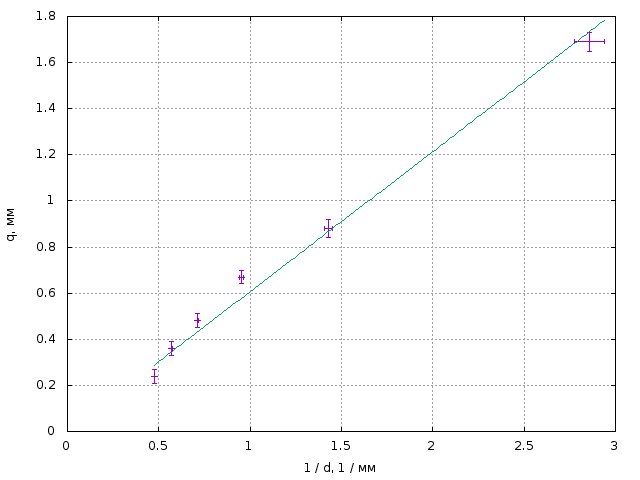
\includegraphics[width = 14cm, height = 7cm]{plot1.png}
\end{figure}
\par
	По коэффициенту наклона прямой графика $\beta$, найденному с помощью метода наименьших квадратов, найдём среднюю длину волны света лампы $\lambda_0$ как
\[
	\lambda_0 = \frac{\beta}{S}
\]
\par
	Погрешность определения $\lambda_0$ мы найдём как (пренебрегая при этом погрешностью $S$ по сравнению с погрешностью $\beta$)
\[
	\Delta_\text{$\lambda_0$} = \frac{\Delta_\beta}{S}
\]
\par
	Полученный коэффицент наклона графика $\beta$
\[
	\beta = \left(0.607 \pm 0.016 \right) \, \text{мм}^2
\]
\par
	Откуда средняя длина волны света лампы
\[
	\lambda_0 = \left(578 \pm 16 \right) \, \text{нм}
\]
\par
	Максимальный порядок интерференционной картины 
\[
	m_\text{ког} = 5
\]
\par
	Следовательно,
\[
	\Delta \lambda = \left(116 \pm 4\right) \, \text{нм}
\]
\par
	Длина когеренции
\[
	\Delta_\text{ког} = \left(2.89 \pm 0.08 \right) \, \text{мкм}
\]
\par
	Время когеренции
\[
	\tau_\text{ког} = \left(0.96 \pm 0.03 \right) \cdot 10^{-14} \, \text{с}
\]
\par
	При рассчёте были использованы формулы, представленные в теоритической части работы. Из них же очевидным образом были получены формулы для рассчёта погрешностей.

\section*{Выводы}
\par
	В ходе работы была оценена длина волны полупроводникового лазера-указки зелёного цвета. Однако точность этой оценки оставляет желать лучшего, так как вместо расстояния между наиболее отдалёнными интерференционными полосами было измерено расстояние между двумя соседними. Также был настроен интерферометр и были определены: средняя длина волны источника света, ширина его спектра излучения, а также длина когеренции и время когеренции.
\par
	Полученная средняя длина волна лампы соответствует диапазону длин волн, соответствующих жёлтому спектральному свету.
\par
	Наибольшую трудность при выполнении данной работы составила настройка интерферометра, а также последующая поддержка его в готовом для работы состоянии.

\end{document}